% Compilare con PDFLaTeX
\documentclass[10pt,final]{siamltex}
\usepackage{graphicx}
\usepackage{latexsym}
\usepackage{amsmath,amssymb}
%\usepackage{gensymb}
\textwidth = 16cm
\usepackage{pstricks}
%\usepackage{subcaption}
\usepackage{algorithm}
\usepackage{algpseudocode}
\usepackage[breakable]{tcolorbox}
\usepackage{doi}
%
\begin{document}
\title{Glomerular filtration rate estimation by a novel binning-less bivariate isotonic statistical regression method}
\author{Sebastian~Giles, Simone~Fiori%
\thanks{S. Giles is with the School of Information and Automation Engineering, 
        Universit\`{a} Politecnica delle Marche, 
        Via Brecce Bianche, I-60131 Ancona (Italy). 
        \newline\indent
        S. Fiori is with Dipartimento di Ingegneria dell'Informazione, 
        Universit\`{a} Politecnica delle Marche, 
        Via Brecce Bianche, I-60131 Ancona (Italy). 
        \newline\indent
        This draft is dated \today.}}
\maketitle
\def\bbbr{\mathbb{R}}
\def\bbbx{\mathbb{X}}
\def\bbby{\mathbb{Y}}
\def\mdef{{\stackrel{{\mathrm{def}}}{=}}}
% Footnotes in non-numerical fashion
\renewcommand*{\thefootnote}{\fnsymbol{footnote}}
\def\to{\mathbf{\ to\ }}
\setcounter{footnote}{1}
%
%
\begin{abstract}
{\red L'abstract contiene un riassunto molto stringato del problema affrontato, dell'applicazione e dei risultati.}
\end{abstract}
%
\section{Introduction}
%
{{\red L'introduzione deve fornire gli elementi, senza addentrarsi nelle formule e nei dettagli tecnici, per capire il problema affrontato e l'applicazione. Questa e' la sezione piu' ``letteraria'' del documento. In questo caso, si puo' parlare in generale della regressione isotonica (= monotona), della sua versione statistica, anche usando parti dell'articolo \cite{fiori} e di altre fonti, e dell'idea di sostituire i passaggi pdf-cdf con un unico passaggio eliminando anche il binning. Si puo' poi parlare dell'applicazione, ovvero dell'importanza del parametro GFR per verificare la funzionalita' renale, della difficolta' di misurare effettivamente questo parametro e della conseguente necessita' pratica di determinare un modello basato su elementi facilmente misurabili quali eta', peso e altezza, facendo riferimento al materiale contenuto in \cite{gfr_plos_one} e in altre fonti.}

The present report is organized as follows. Section~\ref{sec2} recalls the notion of bivariate statistical regression and explains the main idea and the details about the proposed binning-less bivariate statistical regression algorithm. Section~\ref{sec3} explains an analysis of the glomerular-filtration-rate (GFR) estimation based on creatinine levels and illustrates such analysis by means of numerical tests performed on a dataset drawn from a study on pediatric patients in mainland China. Section~\ref{sec4} concludes the paper.
%
\section{Binning-less bivariate statistical regression algorithm}\label{sec2}
%
{{\red Questa sezione spiega i dettagli matematici e tecnici del nuovo algoritmo. Sotto ho riportato, a titolo di esempio, lo pseudo-codice relativo alla mia versione di SBR e i relativi commenti.}

A pseudo code for the proposed function is as in Algorithm~\ref{staircase_algo_mi}. The main idea to avoid binning is to estimate the cumulative distribution function of the two datasets without resorting to an estimate of the probability density function first. We recall from our previous work that, denoting by $P_x(x)$ the CDF of the dataset $X$ and by $P_y(y)$ the CDF of the dataset $Y$, the model is given by $f(x)=P_y^{-1}(P_x(x))$ in case of monotonically increasing relationships, and by $f(x)=P_y^{-1}(1-P_x(x))$ in case of monotonically decreasing relationships. We further recall that, since the modeling solution is not unique, in general, we assumed that the center of mass of the $X$ data corresponds to the center of mass of the $Y$ data.

Note that histogram estimation is used only in conjunction with unique-value extraction and is used only to deal with repeated values, therefore, there's actually no binning in the procedure, as opposed to our previous methods.
Also, note that that this procedure works only for monotonic models (for non-monotonic data\-sets/mo\-del, we would need to resort to data pre-monotonization \cite{fgl}). In particular, the pseudo-code in Algorithm~\ref{staircase_algo_mi} is suitable for \textit{monotonically increasing} models. 

%
\begin{algorithm}[t]
\caption{Staircase regression: Monotonically increasing}
\label{staircase_algo_mi}
\begin{algorithmic}[1]
\Function{staircaseRegression}{$X$, $Y$, $x_q$}
    
    \State $N \gets$ \textbf{lenght}$(X)$ 
    \Comment Get cardinality of data set $X$
    
    \State $(R_x,X_s) \gets \textbf{hist}(X,\textbf{unique}(X))$
    \Comment Compute the number of repetitions in $X$ and the unique values in $X$

    \State $P_x \gets \mathbf{cumsum}(R_x)/N$
    \Comment Estimate the CDF of the dataset $X$
    
    \State $c \gets \mathbf{sum}(X_s \leq x_q)$
    \Comment $X_s[c]$ is the (unique) larger value in the dataset $X$ smaller than (or equal to) the query point $x_q$

    \If{$c = \mathbf{length}(X_s)$}
      \State $P_{xq} \gets 1$
    \Else 
      \State $P_{xq} \gets P_x[c] + (P_x[c+1]-P_x[c])*(x_q-X_s[c])/(X_s[c+1]-X_s[c])$
    \EndIf
    \Comment Estimate the value of the CDF of $X$ at the query point $x_q$ by linear interpolation
    
    \State $M \gets$ \textbf{lenght}$(Y)$ 
    \Comment Get cardinality of data set $Y$  
    
    \State $(R_y,Y_s) \gets \textbf{hist}(Y,\textbf{unique}(Y))$
    \Comment Compute the number of repetitions in $Y$ and the unique values in $Y$

    \State $P_y \gets \mathbf{cumsum}(R_y)/M$
    \Comment Estimate the CDF of the dataset $Y$
    
    \State $c \gets \mathbf{sum}(P_y \leq P_{xq})$
    \Comment $Y_s[c]$ is the (unique) value in the dataset smaller or equal to the query point $y_q$ yet to be determined
    
    \If{$c = \mathbf{length}(Y_s)$}
        \State $y_q \gets Ys[c]$
    \Else
        \State $y_q \gets Y_s[c] + (P_{xq} - P_y[c])*(Y_s[c+1]-Y_s[c])/(P_x[c+1]-P_x[c])$
    \EndIf
    \State \textbf{return} $y_q$
\EndFunction
\end{algorithmic}
\end{algorithm}
%

Here are a few comments on the pseudo-code:
%
\begin{itemize}
\item \textbf{Line 2}: The variable $N$ contains the number of data-points in the array $X$.
\item \textbf{Line 3}: As we know, it will return $X_s \gets \mathbf{unique}(X)$, namely, the array $X_s$ will contain the unique values coming from the array $X$, sorted in ascending order. Now, $\mathbf{hist}(X,X_s)$ counts how many times the values in $X$ equal the values in $X_s$, namely, how many times each unique value is repeated in $X$. The list of repetitions is saved in the array $R_x$. For example, if the array $X$ contains no repetitions, $X_s$ will just be a sorted version of $X$ while all the values in $R_x$ will equal $1$.
\item \textbf{Line 4}: The cumulative sum of all repetitions, normalized by the total number of samples $N$, will give an estimation of the cumulative distribution function of the dataset $X$. The first value of the CDF is $0$ by default so we do not store it.
\item \textbf{Line 5}: The CDF is stored in the array $P_x$ and is conceptually a staircase approximation. If the query coordinate $x_q$ does not belong to the dataset $X$ (likely it won't), we do not know the value of the CDF at $x_q$ (let us denote it by $P_{xq}$). The simplest method to approximate the value of the CDF at $x_q$ is by linear interpolation. First, we look for the (unique) value in the dataset that is smaller than, or equal to, the value $x_q$. The variable $c$ will contain the index of the element in the array $X_s$ corresponding to such value.
\item \textbf{Line 6--10}: If the counter $c$ points to the last entry in the array, then set $P_{xq}=1$ because we cannot go beyond this point. If the counter $c$ points to the middle of the array, approximate $P_{xq}$ by a linear interpolation, which arises as the solution of the linear equation $\tfrac{x_q-X_s[c]}{X_s[c+1]-X_s[c]}=\tfrac{P_{xq}-P_x[c]}{P_x[c+1]-P_x[c]}$.
\item \textbf{Line 11}: The variable $M$ contains the number of data-points in the array $Y$.
\item \textbf{Line 12-13}: Returns an estimation of the cumulative distribution function of the dataset $Y$ similarly to what has been done for the dataset $X$.
\item \textbf{Line 14}: The staircase approximation of the CDF is stored in the array $P_y$. Let us denote the value of the CDF at the (unknown) point $y_q$ as $P_{yq}$. By definition, $y_q$ is the $y$-coordinate corresponding to the $x$-coordinate $x_q$ if $P_{xq} = P_{yq}$. The equality is not exactly verified, in practice, therefore we first identify the value of $P_y$ which is smaller than, or equal to, $P_{xq}$, pointed by the index $c$.
\item \textbf{Line 15--19}: If $c$ points to the end of the array, then set $y_q$ as the largest value in the dataset $Y_s$ (since the values are sorted in ascending order, the largest value corresponds to the tail of the array), because we cannot go beyond this point. If $c$ points to the middle of the array, approximate $y_q$ by a linear interpolation, which arises as the solution of the equation $\tfrac{y_q-Y_s[c]}{Y_s[c+1]-Y_s[c]}=\tfrac{P_{xq}-P_y[c]}{P_y[c+1]-P_y[c]}$.
\end{itemize}

Note that the code strictly deals with \emph{interpolation}, namely, it is supposed that $\min\{X\}\leq x_q \leq \max\{X\}$.

%\noindent\fcolorbox{blue}{lightgray}{%
%    \minipage[h]{\dimexpr\linewidth-2\fboxsep-2\fboxrule\relax}
\begin{tcolorbox}[colback=gray!30,%gray background
                  colframe=black,% black frame colour
                  width=\dimexpr\linewidth-2\fboxrule\relax,
                  arc=3mm, auto outer arc, 
                  breakable
                 ]
\underline{\textsc{Small numerical example}}: Let $X=[4,1,4,2,3,1,1,2]$ and $Y=[10,     4,    {\red 5},10,     6,     8,     4,     4,     6]$, i.e., $N=8$, $M=9$. The actual underlying model is $f(x)=2x+2$. Note that the data aren't paired and there's an extra datum in $Y$ (in red). Let the query point be $x_q=\tfrac{5}{2}$. Then, the pseudo-code computes:
%
\begin{eqnarray*}
&& X_s = [1,     2,     3,     4]\\
&& R_x = [3,     2,     1,     2]\\
&& P_x = [\tfrac{3}{8}, \tfrac{5}{8}, \tfrac{6}{8}, 1]\\
&& c = 2.
\end{eqnarray*}
%
By linear interpolation, the pseudo-code computes 
%
\begin{equation*}
P_{xq}=\frac{5}{8}+\frac{\left(\tfrac{6}{8}-\tfrac{5}{8}\right)\left(\tfrac{5}{2}-2\right)}{3-2}=\frac{11}{8}.
\end{equation*}
%
Further, the pseudo-code computes:
%
\begin{eqnarray*}
&& Y_s = [4,     5,     6,     8,    10]\\
&& R_y = [3,     1,     2,     1,     2]\\
&& P_y = [\tfrac{3}{9}, \tfrac{4}{9}, \tfrac{6}{9}, \tfrac{7}{9}, 1]\\
&& c = 3.
\end{eqnarray*}
%
By a further linear interpolation, the pseudo-code computes 
%
\begin{equation*}
y_q = 6 + \frac{\left(\tfrac{11}{16}-\tfrac{6}{9}\right)\left(8-6\right)}{\tfrac{7}{9}-\tfrac{6}{9}}=\frac{51}{8},
\end{equation*}
%
that is, $y_q\approx 6.375$, while the exact value would be $2x_q+2=7$.

It is interesting to see that, if we take off the extra `5' datum from the set $Y$, the pseudo-code will return exactly $y_q=7$!
%\endminipage}
\end{tcolorbox}
%
\section{Application to glomerular filtration rate estimation}\label{sec3}
%
{{\red Questa sezione presenta i dati, le loro rappresentazioni grafiche, i risultati delle regressioni, i confronti con i modelli analitici, e i relativi commenti esplicativi. Qui vanno spiegati anche gli indici di prestazione MSE e Roughness. Per quest'ultimo, si puo' fare riferimento alla regolarizzazione di Tikhonov riassunta in \cite{bishop}. Le figure, fatte con MATLAB, possono essere salvate in formato PDF e caricate all'interno del documento come mostrato sotto. Idem per la tabella che può essere salvata dal MATLAB direttamente in formato LaTeX.}}

An example of result of application of the Algorithm~\ref{staircase_algo_mi} to a real-world dataset is shown in the Figure~\ref{bodyfat}.

\vspace{5mm}
%
\begin{figure}[h!]
\centering
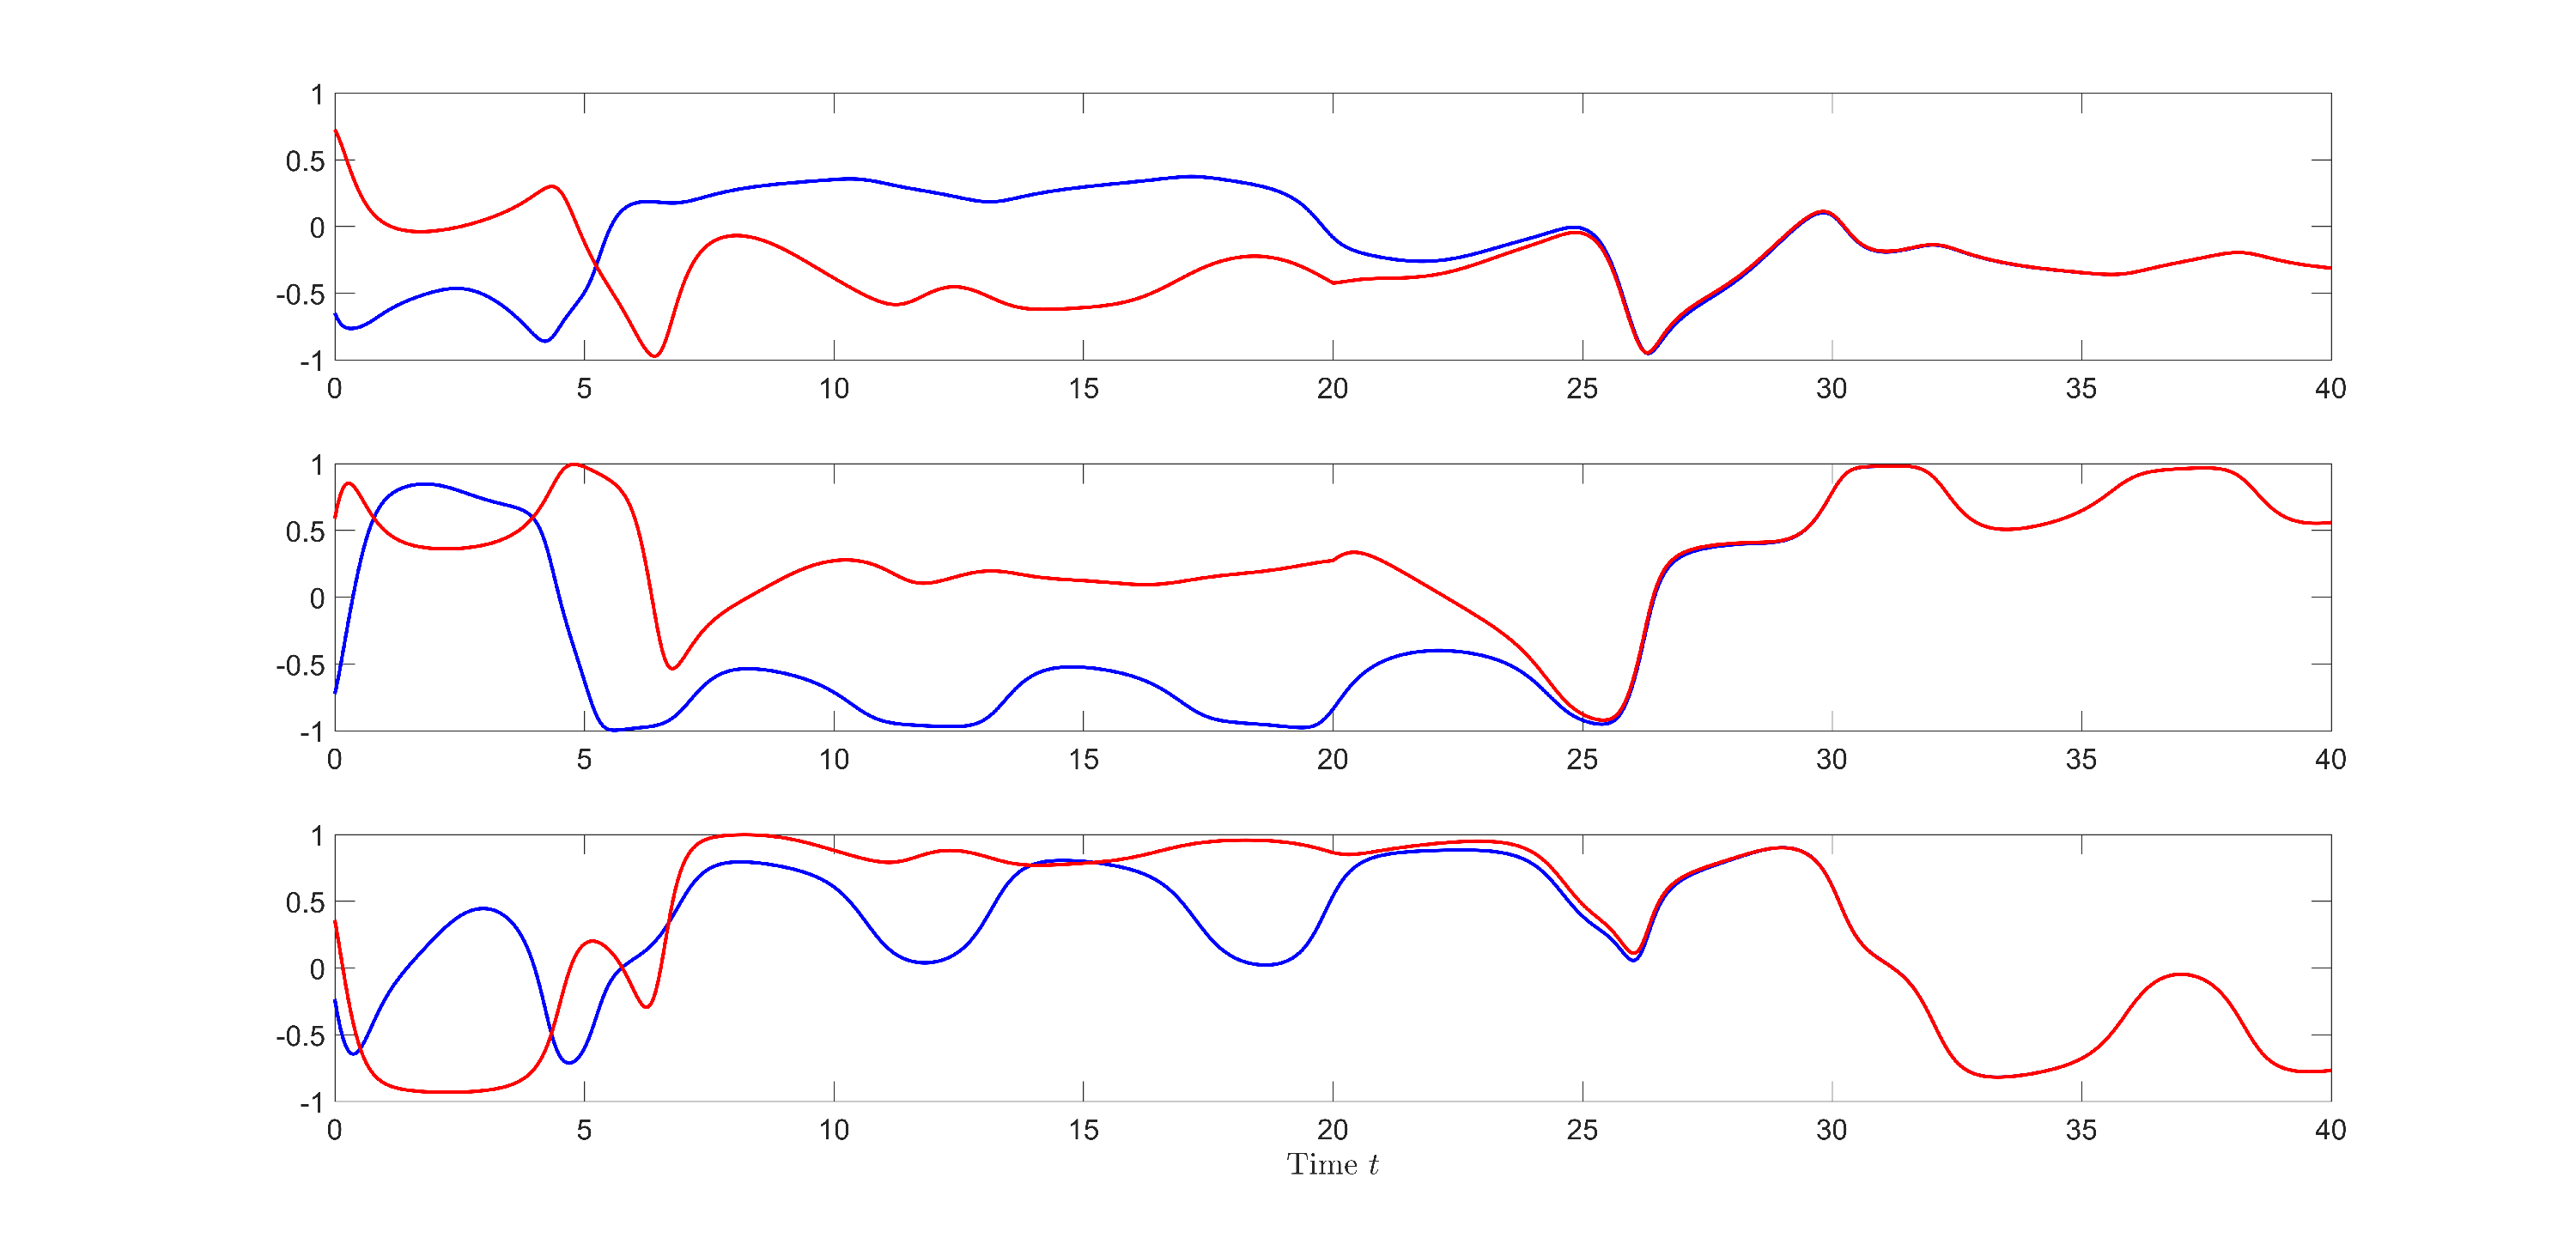
\includegraphics[scale=0.3]{Experiment1a}
\caption{Example of figure.}
\label{bodyfat}
\end{figure}
%
%
\section{Conclusions}\label{sec4}
%
{{\red Questa sezione riassume i risultati, sia concettuali che pratici, ottenuti.}}
%
\begin{thebibliography}{99}
%
\bibitem{bishop} C.M. Bishop, ``Training with noise is equivalent to Tikhonov regularization'', \textit{Neural Computation}, Vol. 7, No. 1, pp. 108 -- 116, 1995
\bibitem{fiori} S. Fiori, ``Fast statistical regression in presence of a dominant independent variable'', \textit{Neural Computing and Applications}, Vol. 22, No. 7, pp. 1367 -- 1378, 2013
\bibitem{fgl} S. Fiori, T. Gong and H.K. Lee, ``Bivariate nonisotonic statistical regression by a lookup table neural system'', \textit{Cognitive Computation}, Vol. 7, No. 6, pp. 715 -- 730, 2015
\bibitem{gfr_plos_one} K. Zheng, M. Gong, Y. Qin, H. Song, X. Shi, Y. Wu, F. Li and X. Li, ``Validation of glomerular filtration rate-estimating equations in Chinese children'', \textit{PLoS ONE}, Vol. 12, No. 7, pp. e0180565 (\doi{10.1371/journal.pone.0180565}), 2017
%
\end{thebibliography}
\end{document}
